\subsubsection{UC14 - Gestione ordini}
\begin{figure}[h]
	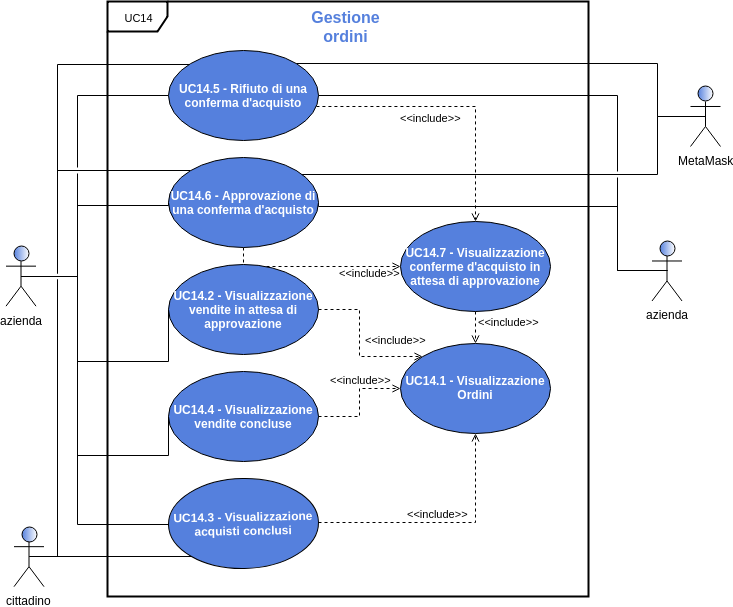
\includegraphics[width=10cm]{res/images/UC14-GestioneOrdini.png}
	\centering
	\caption{Gestione degli ordini}
\end{figure}
\begin{itemize}
	\item \textbf{Attori Primari}: azienda, cittadino;
	\item \textbf{Descrizione}: agli utenti sono messe a disposizione diverse operazione per visualizzare e gestire gli ordini;
	\item \textbf{Scenario principale}: l'utente visualizza e svolge alcune operazioni per gestire gli ordini dei quali ne è partecipe;
	\item \textbf{Precondizione}: il sistema ha riconosciuto l'utente autenticato come azienda o cittadino e mette a disposizione tutte le pagine necessarie alla visualizzazione e gestione degli ordini;
	\item \textbf{Postcondizione}: l'utente ha visualizzato e/o gestito i propri ordini.
\end{itemize} 
\subsubsection{UC14.1 - Visualizzazione Ordini}
\begin{itemize}
	\item \textbf{Attori Primari}: azienda, cittadino;
	\item \textbf{Descrizione}: alle aziende ed ai cittadini sono messe a disposizione diverse operazione per visualizzare e gestire gli ordini all'interno della piattaforma. In tale maniera vi è possibile avere un elenco dettagliato di tutti gli ordini, in particolare:
	\begin{itemize}
		\item visualizzazione data dell'ordine;
		\item visualizzazione numero dell'ordine;
		\item visualizzazione prezzo netto;
		\item visualizzazione prodotti inclusi nell'ordine;
		\item visualizzazione totale IVA;
		\item visualizzazione prezzo lordo;
	\end{itemize}
	\item \textbf{Scenario principale}: l'utente visualizza e svolge alcune operazioni per gestiregli ordini;
	\item \textbf{Precondizione}: il sistema ha riconosciuto l'utente autenticato come azienda o cittadino e mette a disposizione tutte le pagine necessarie alla visualizzazione e gestione degli ordini;
	\item \textbf{Postcondizione}: l'utente ha visualizzato e/o gestito i propri ordini.
\end{itemize} 

\subsubsection{UC14.2 - Visualizzazione vendite in attesa di approvazione}
\begin{itemize}
	\item \textbf{Attori Primari}: azienda;
	\item \textbf{Descrizione}: all'azienda è messa a disposizione la possibilità di visualizzare e gestire le vendite in attesa di approvazione;
	\item \textbf{Scenario principale}: l'utente visualizza le vendite in attesa di approvazione tramite una vista dettagliata che include: 
		\begin{itemize}
		\item visualizzazione data ultima per la conferma;
	\end{itemize}
		\item \textbf{Inclusioni}:
	\begin{itemize}
		\item \textbf{UC14.1}: Visualizzazione degli ordini;
	\end{itemize}
	\item \textbf{Precondizione}: il sistema ha riconosciuto l'utente autenticato come azienda e mette a disposizione tutte le pagine necessarie alla visualizzazione di questo tipo di ordini;
	\item \textbf{Postcondizione}: l'utente ha visualizzato e/o gestito le rpoprie vendite in attesa di approvazione.
\end{itemize} 

\subsubsection{UC14.3 - Visualizzazione acquisti conclusi}
\begin{itemize}
	\item \textbf{Attori Primari}: cittadino, azienda;
	\item \textbf{Descrizione}: l'utente può visualizzare la lista degli acquisti conclusi;
	\item \textbf{Scenario principale}: l'utente visualizza la lista degli acquisti conclusi;
	\item \textbf{Inclusioni}:
	\begin{itemize}
		\item \textbf{UC14.1}: Visualizzazione degli ordini;
	\end{itemize}
	\item \textbf{Precondizione}: il sistema ha riconosciuto l'utente autenticato come azienda o cittadino e questo ha espresso la volontà di visualizzare la lista degli acquisti conclusi;
	\item \textbf{Postcondizione}: l'utente visualizza tale lista.
\end{itemize}

\subsubsection{UC14.4 - Visualizzazione vendite concluse}
\begin{itemize}
	\item \textbf{Attori Primari}: azienda;
	\item \textbf{Descrizione}: l'utente può visualizzare la lista delle proprie vendite ritenute concluse;
	\item \textbf{Scenario principale}: l'utente visualizza la lista delle vendite concluse;
	\item \textbf{Inclusioni}:
	\begin{itemize}
		\item \textbf{UC14.1}: Visualizzazione degli ordini;
	\end{itemize}
	\item \textbf{Precondizione}: il sistema ha riconosciuto l'utente autenticato come azienda e questo ha espresso la volontà di visualizzare la lista delle vendite concluse;
	\item \textbf{Postcondizione}: l'utente visualizza tale lista.
\end{itemize}


\subsubsection{UC14.5 - Rifiuto di una proposta di acquisto}
\begin{itemize}
	\item \textbf{Attori Primari}: azienda;
	\item \textbf{Attori Secondari}: MetaMask\glo, azienda;
	\item \textbf{Descrizione}: l'azienda può rifiutare una proposta d'acquisto. Per confermare l'operazione verrà utilizzato MetaMask\glo;
	\item \textbf{Scenario principale}: l'utente visualizza una proposta d'acquisto che necessitano di conferma e decide di rifiutarla;
	\item \textbf{Inclusioni}: 
	\begin{itemize}
		\item \textbf{UC14.7}: visualizzazione delle proposte d'acquisto in attesa di approvazione;
	\end{itemize}
	\item \textbf{Precondizione}: il sistema ha riconosciuto l'utente autenticato come azienda ed ha mostrato la lista delle proposte d'acquisto che necessitano di conferma;
	\item \textbf{Postcondizione}: l'azienda ha rifiutato la proposta d'acquisto. La proposta non sarà più presente nella lista di attesa per la conferma. L'acquisto comparirà come acquisto concluso, con esito negativo, nella lista delle vendite dell'azienda-venditrice [UC14.4]. Il sistema ritorna l'ammontare trattenuto per l'ordine all'azienda-cliente.
\end{itemize}
\subsubsection{UC14.6 - Conferma di una proposta di acquisto}
\begin{itemize}
	\item \textbf{Attori Primari}: azienda;
	\item \textbf{Attori Secondari}: MetaMask\glo, azienda;
	\item \textbf{Descrizione}: l'azienda accetta la proposta d'acquisto ricevuta;
	\item \textbf{Scenario principale}: l'azienda decide di approvare una proposta d'acquisto da parte di un acquirente. L'utente acquirente ha la possibilità di effettuare il versamento all'azienda-venditrice;
		\item \textbf{Inclusioni}: 
	\begin{itemize}
		\item \textbf{UC14.7}: visualizzazione delle proposte d'acquisto in attesa di approvazione;
	\end{itemize}
	\item \textbf{Precondizione}: il sistema ha riconosciuto l'utente autenticato come azienda, e questo ha espresso la volontà di approvare una richiesta d'acquisto;
	\item \textbf{Postcondizione}: l'azienda approva tale proposta.
\end{itemize}


\subsubsection{UC14.7 - Visualizzazione proposte d'acquisto in attesa di approvazione}
\begin{itemize}
	\item \textbf{Attori Primari}: azienda;
	\item \textbf{Descrizione}: l'azienda può visualizzare delle proposte d'acquisto che necessitano di conferma;
	\item \textbf{Scenario principale}: l'utente visualizza la lista delle proposte d'acquisto che necessitano di conferma. Per ognuna di esse ha a possibilità di confermare la proposta [UC14.6] o di rifiutarla [UC14.5];
		\item \textbf{Inclusioni}:
	\begin{itemize}
		\item \textbf{UC14.1}: Visualizzazione degli ordini;
	\end{itemize}
	\item \textbf{Precondizione}: il sistema ha riconosciuto l'utente autenticato come azienda e questo ha espresso la volontà di visualizzare la lista delle proposte d'acquisto che necessitano di conferma;
	\item \textbf{Postcondizione}: l'azienda visualizza tale lista.
\end{itemize}





